\texit{Определение} Адаптер

Низкоранговый адаптер Lora работает путем сжатия 
параметров модели с использованием низкоранговых матриц. 
Основная идея заключается в том, 
чтобы аппроксимировать исходные параметры модели с
помощью матриц меньшего ранга, что позволяет снизить объем памяти.
Это позволяет снизить объем памяти,необходимый для хранения параметров и ускорить вычисления. 


Наиболем популярным вариантом адаптера является Lora \cite{hu2021lora}, применяющая не только 

Задание верхней границе ранга адаптера выполняется через произведение 

Пусть $W$ - исходная матрица параметров модели размером
 $m \times n$, где $m$ - число входных признаков, 
 а \( n \) - число выходных нейронов.
Тогда для аппроксимации матрицы $W$ с
помощью низкоранговой матрицы $W_{\text{low}}$
размерности \( m \times r \) и \( H \) размерности \( r \times n \) (где \( r \) - это ранг аппроксимации) используется следующая формула:



\begin{figure}[h]
    \centering
    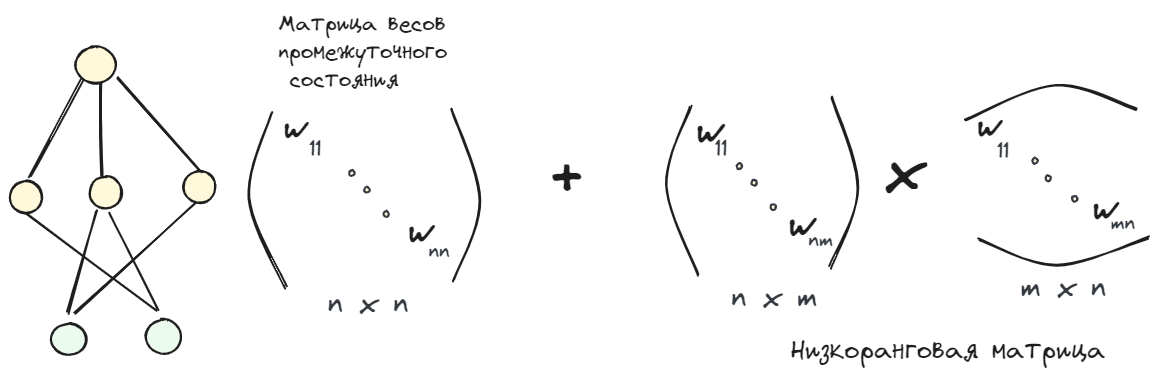
\includegraphics[width=0.5\textwidth]{assets/ml/adapter/adapter.excalidraw.png}
    \caption{Модель адаптера \cite{stablediffusion}}
    \label{sd_learning}
\end{figure}



Для любых матрица $A$ и $B$ выполняется
$$
    \rang(𝐴𝐵) \le \min\left(\rang(𝐴),\rang(𝐵))
$$

$$
    W \approx W_{\text{low}} \cdot H
$$

Здесь \( W_{\text{low}} \) и \( H \) оптимизируются с целью минимизации ошибки аппроксимации между \( W \) и \( W_{\text{low}} \cdot H \), например, с использованием метода наименьших квадратов.

Таким образом, процесс работы низкорангового адаптера Lora заключается в нахождении оптимальных низкоранговых приближений для параметров модели, что позволяет сократить объем памяти и вычислительные затраты при сохранении приемлемого качества предсказания модели.
